\section{КОНСТРУКТОРСКИЙ РАЗДЕЛ}

В разделе описывается метод распознавания суицидальных паттернов поведения человека по текстовым сообщениям, а также формат и метод сбора задействованных в нем данных. 
Приводится диаграмма вариантов использования, декомпозиция задачи распознавания суицидального сообщения, а также диаграмма ``сущность-связь'' в нотации Чена. 
Определяется перечень задействованных методов машинного обучения и векторизации.

\subsection{Формат и метод сбора данных}

В качестве задействованных в анализе данных используются текстовые сообщения и их даты написания, так как представленная зависимость количества смертей от суицида в зависимости от года и месяца говорит о возможной корреляции месяца написания сообщения и его возможной интерпретации.

Для сбора данных задействовано автоматизированное средство сбора суицидальных сообщений в мессенджере Telegram. Интерфейс программного обеспечения позволяет направить в систему хранения два типа сообщений: суицидальные и на суицидальную тематику.

Средство сбора должно предоставлять пользователю следующий функционал:

\begin{enumerate}
\item[1.] Получение информации о проекте;
\item[2.] Получение информации об отличиях суицидальных сообщений и сообщений на суицидальную тематику;
\item[3.] Направление примеров суицидальных сообщений;
\item[4.] Направление примеров сообщений на суицидальную тематику.
\end{enumerate}

Согласно 152-ФЗ ``О персональных данных'', ``персональные данные -- любая информация, относящаяся к прямо или косвенно определенному или определяемому физическому лицу (субъекту персональных данных)'' \cite{fzpers}. Таким образом, к персональным данным можно отнести фамилию, имя и отчество, дату и место рождения, адрес проживания, семейное, социальное и имущественное положение, образование, профессию, доходы и другое. В связи с этим средство сбора информации, не обрабатывает и не хранит никаких персональных данных о пользователях, направивших сообщения.

\subsection{Средства реализации ботов в мессенджере Telegram}

В качестве представленных к использованию в качестве средства реализации бота в мессенджере телеграм могут быть задействованы популярные библиотеки:

\begin{itemize}
	\item Python Telegram Bot \cite{pythonTelegram},
	\item Telebot \cite{telebot},
	\item Node Telegram Bot API \cite{nodeTelegram},
	\item Telegram Bot Kotlin \cite{kotlinTelegram}.
\end{itemize}

Python Telegram Bot -- это библиотека, предоставляющая асинхронный интерфейс на ЯП Python для Telegram Bot API, которая совместима с версиями Python3.8 \cite{Python} и выше. Данная библиотека предоставляет высокий уровень абстракции и позволяет использовать объектно-ориентированный подход. Помимо реализации API, она также содержит ряд классов высокого уровня, упрощающих разработку ботов. Кроме того, проект поддерживает строенную с асинхронным вводом-выводом. \cite{pythonTelegram}

Telebot -- библиотека на Python, содержащая в себе асинхронную и синхронную реализацию Telegram Bot API. Данный проект предоставляет более гибкий и низкоуровневый доступ к API Telegram, чем упомянутый Python Telegram Bot. \cite{telebot}

Node Telegram Bot API -- это библиотека для создания Telegram-ботов с использованием языка JavaScript \cite{js} и платформы NodeJS \cite{nodejs}. Несмотря на распространенное использование, используемая версия API Telegram является устаревшей. \cite{nodeTelegram}

Telegram Bot Kotlin -- это библиотека для создания Telegram-ботов на ЯП Kotlin \cite{Kotlin}. Отличительной особенностью является возможность разработки ботов на платформе Java Virtual Machine \cite{jvm}, а также поддержка Kotlin Coroutines. \cite{kotlinTelegram}

\subsection{Декомпозиция системы}

На рисунке \ref{img:useCase} представлена диаграмма вариантов использования системы.

\begin{figure}[H]
	\centering
	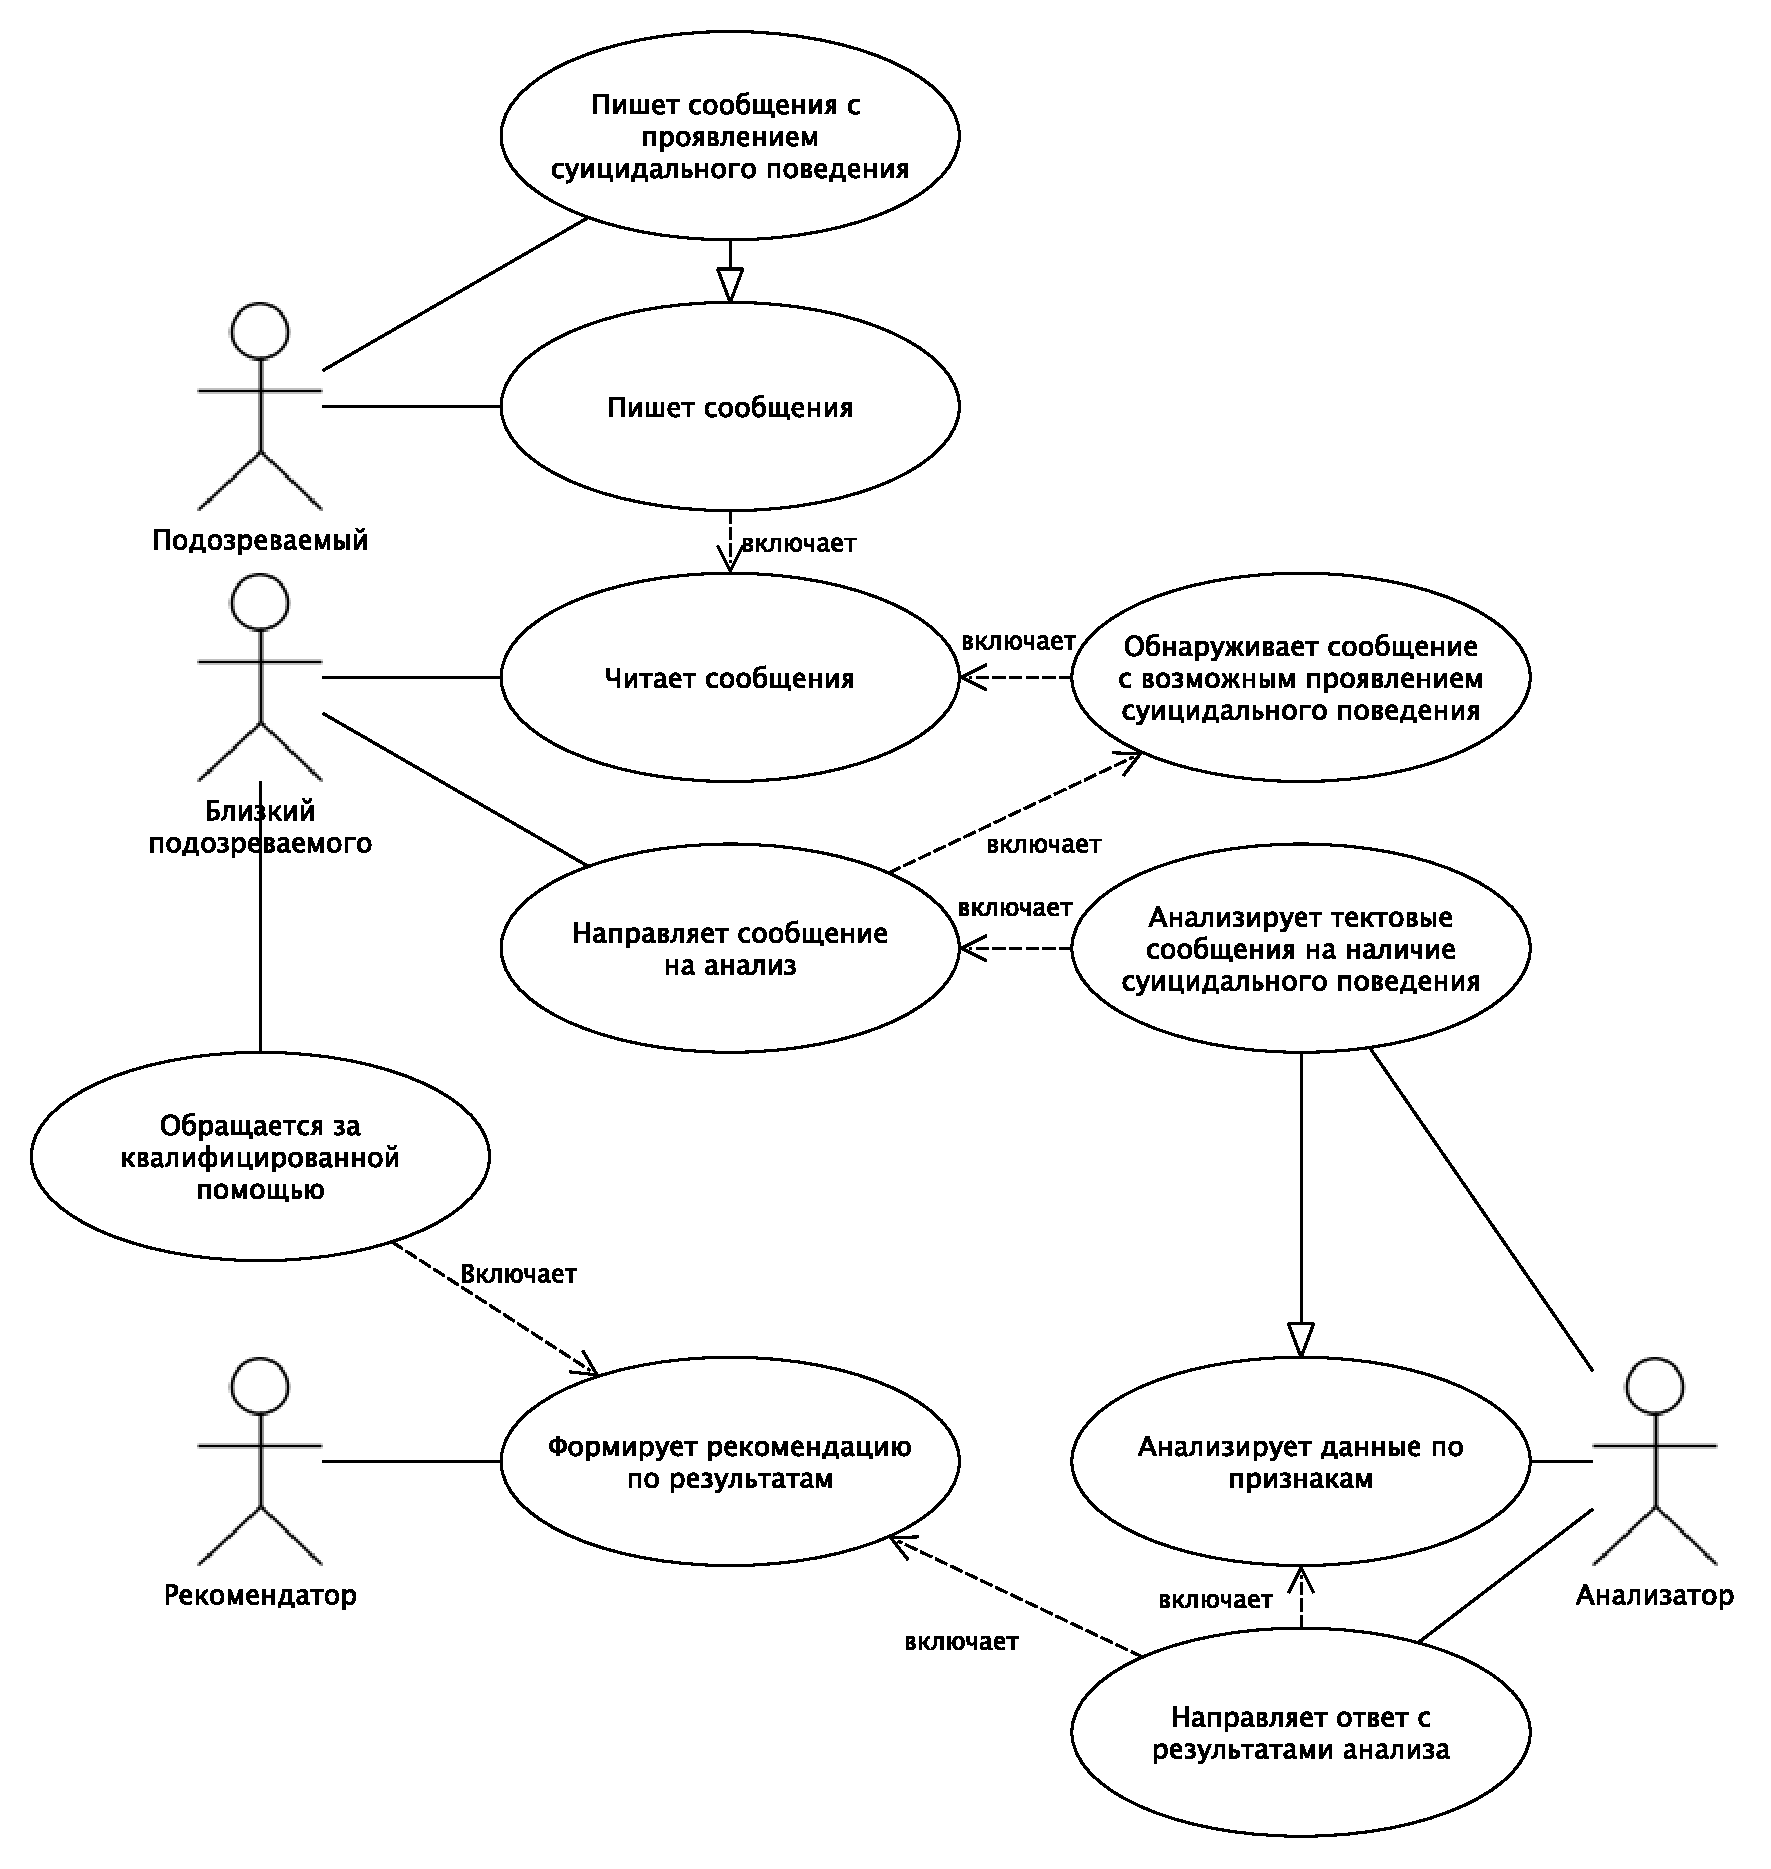
\includegraphics[width=\textwidth]{inc/useCase.pdf}
	\caption{ Диаграмма вариантов использования системы. }
	\label{img:useCase}
\end{figure}

На рисунке \ref{img:idef1} представлена IDEF0 диаграмма первого уровня задачи определения наличия суицидальных паттернов в текстовом сообщении.

\begin{figure}[H]
	\centering
	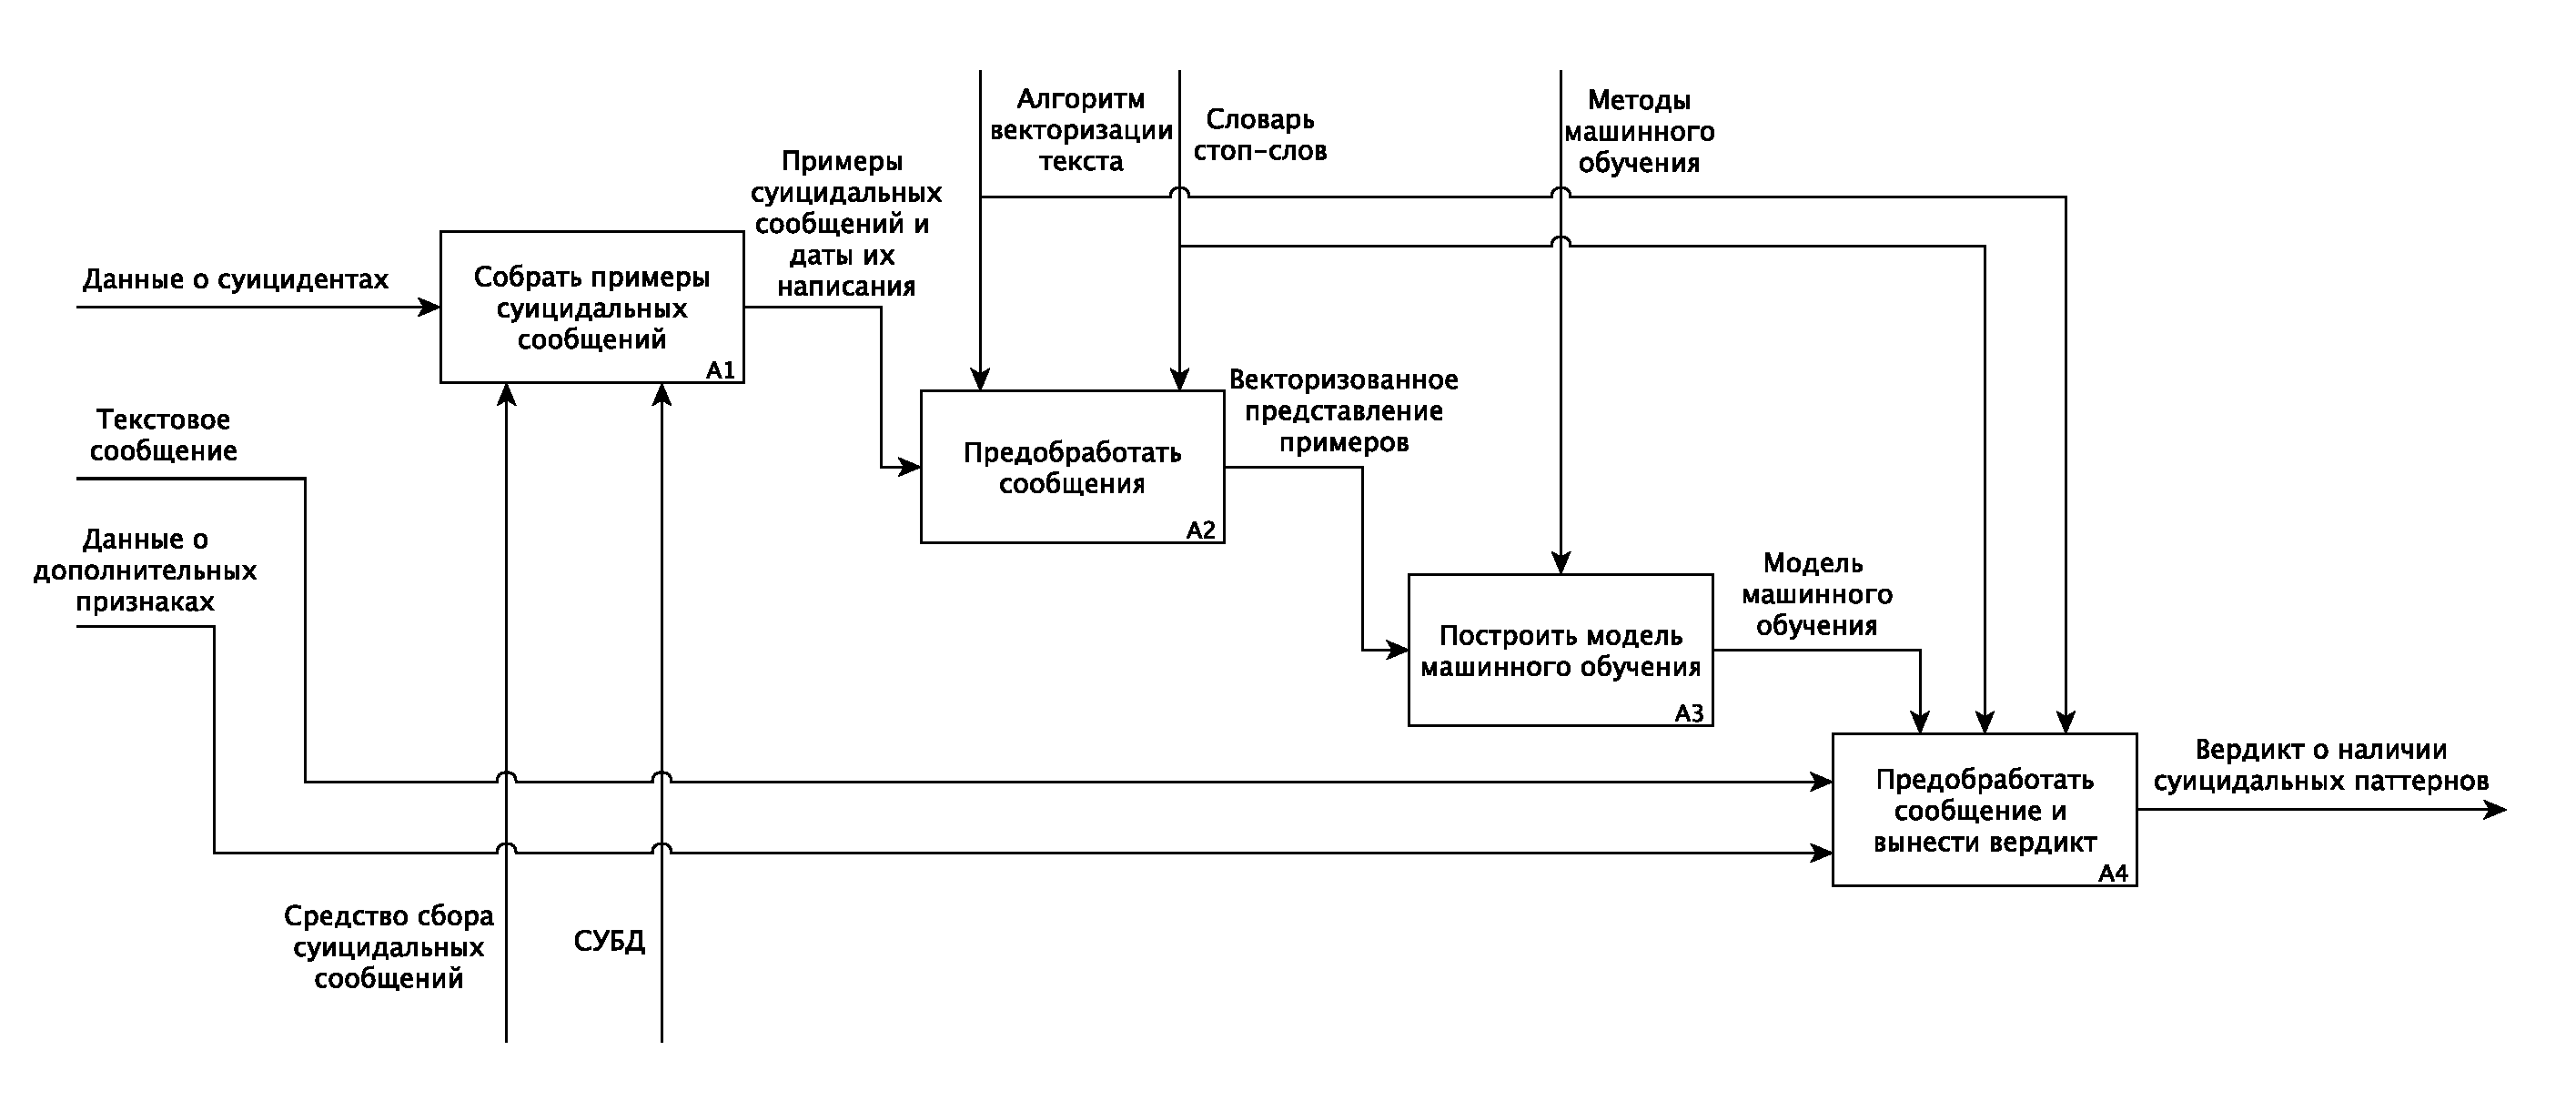
\includegraphics[width=\textwidth]{inc/A1.pdf}
	\caption{ IDEF0 диаграмма первого уровня. }
	\label{img:idef1}
\end{figure}

Модуль А1 на рисунке \ref{img:idef1} отвечает за сбор примеров суицидальных сообщений с использованием средства сбора суицидальных сообщений и СУБД. 
Средство сбора суицидальных сообщений в данном контексте подразумевает программное обеспечение, позволяющее пользователям вносить размеченные сообщения, то есть текст с указанным классом, к которому он относится, для его последующего использования и хранения в базе данных.

Модуль А2 на рисунке \ref{img:idef1} отвечает за предобработку данных, собранных на этапе А1, включающую в себя токенизацию, лемматизацию, удаление стоп-слов и векторизацию.
В результате выполнения блока будет получено векторизованное представление поступивших в него примеров суицидальных сообщений. 
Декомпозиция рассматриваемого блока приведена на рисунке \ref{img:idef21}.

\begin{figure}[H]
	\centering
	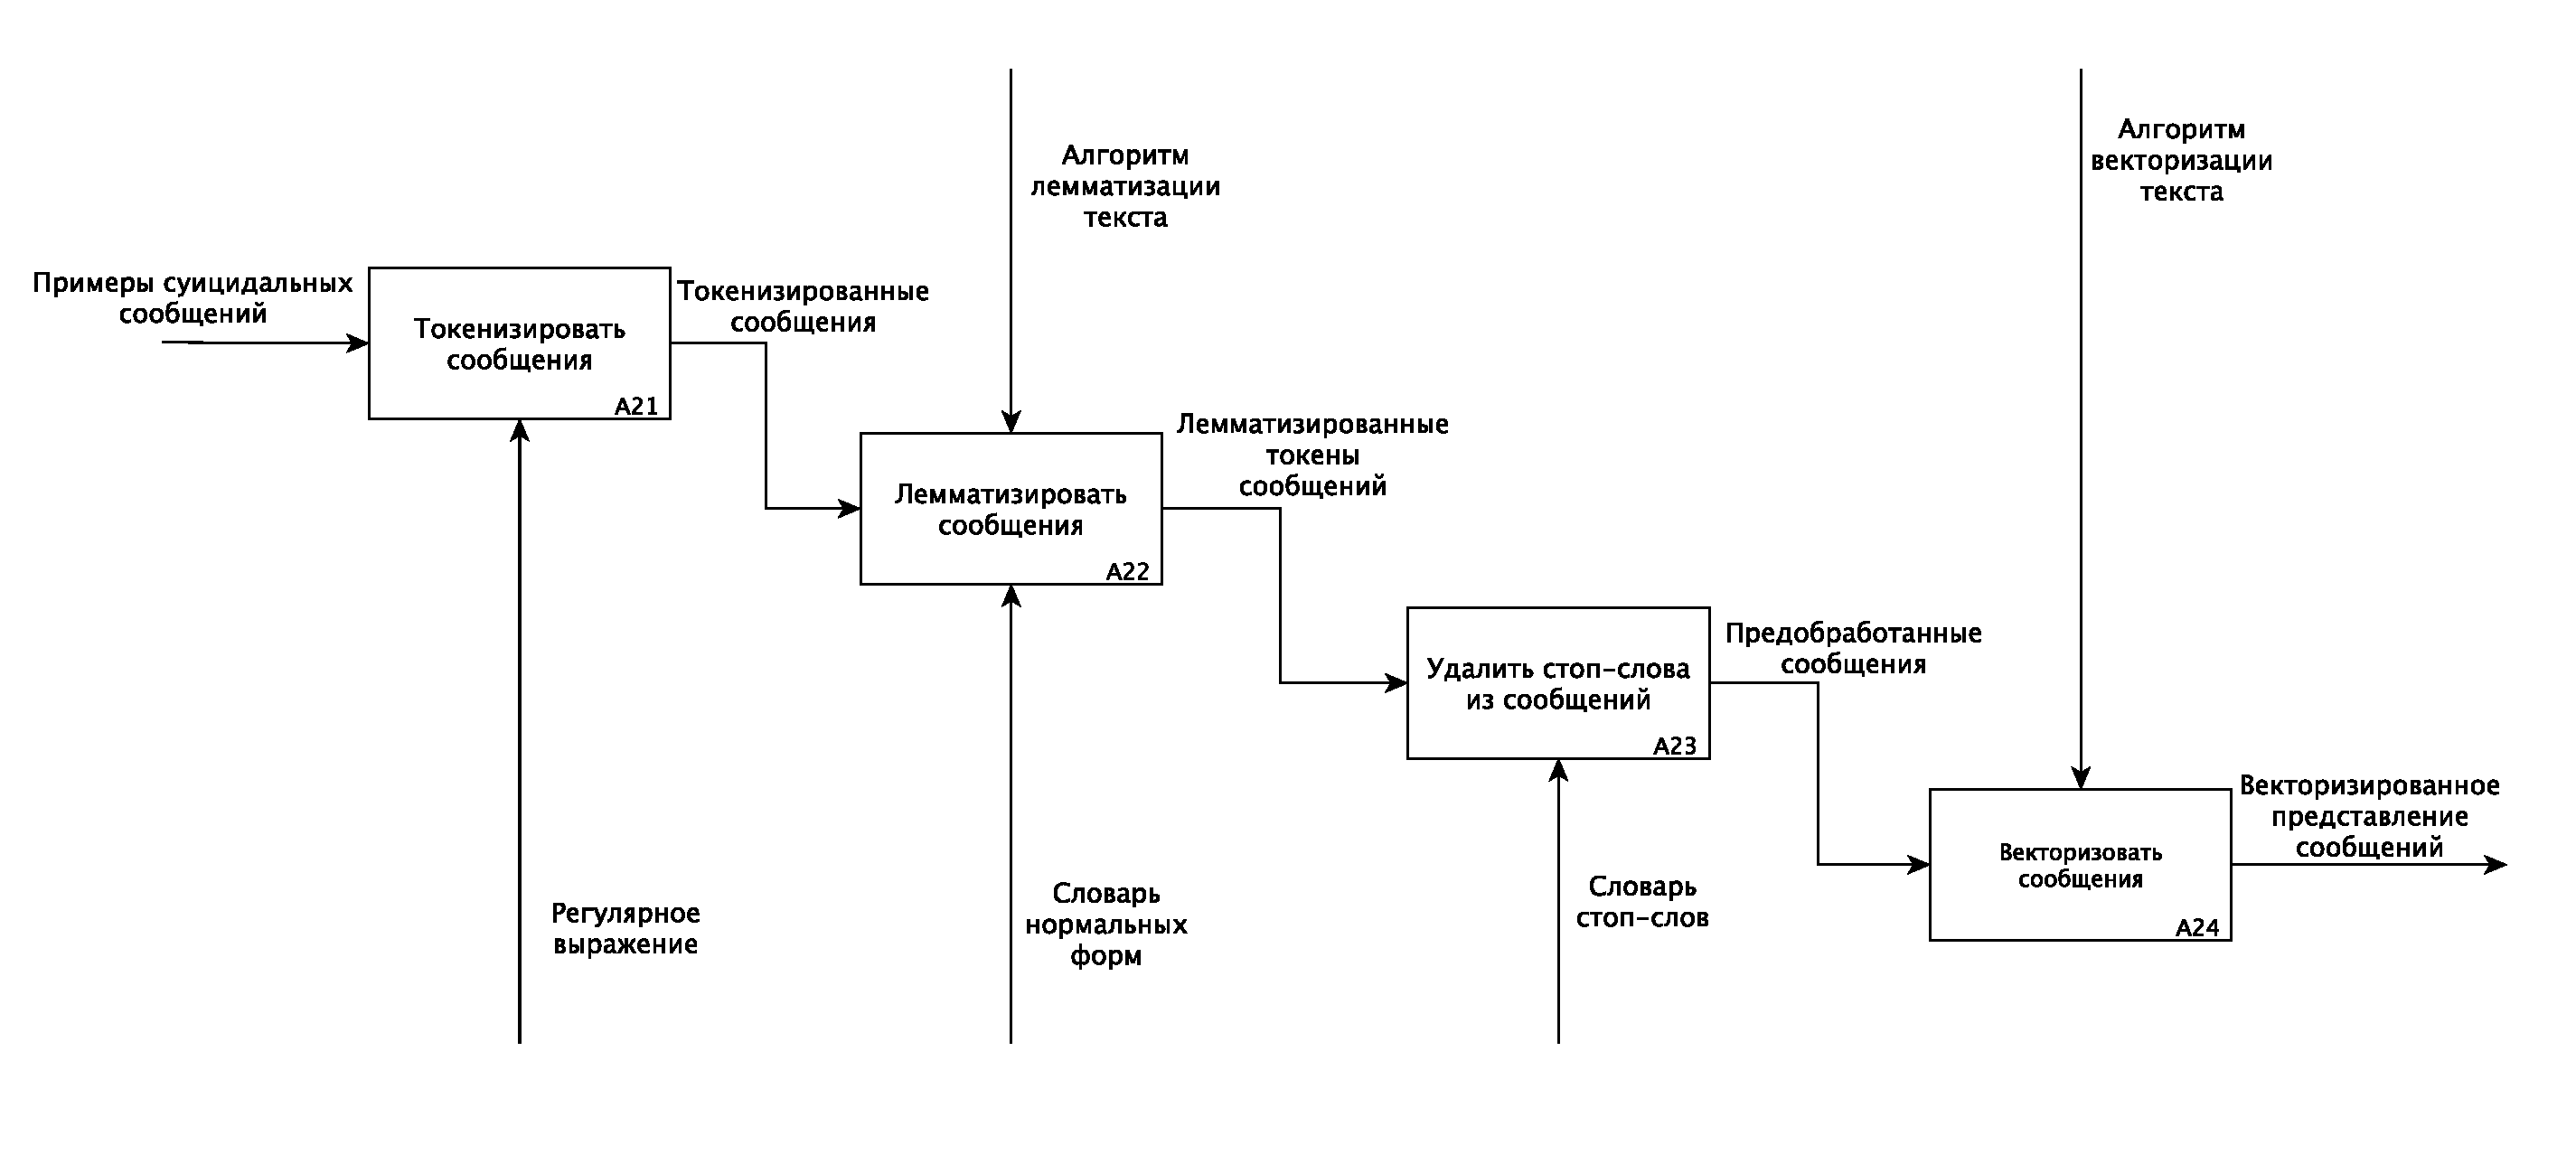
\includegraphics[width=\textwidth]{inc/A21.pdf}
	\caption{ IDEF0 диаграмма, декомпозиция блока A2. }
	\label{img:idef21}
\end{figure}

Модуль А3 на рисунке \ref{img:idef1} отвечает за построение модели машинного обучения, играющую роль классификатора сообщений. 
В качестве контроля блока выстапают методы машинного обучения: градиентный бустинг, метод случайного леса, метод опорных векторов, метод К-ближайших соседей, логистическая регрессия и перцептрон.

Модуль А4 на рисунке \ref{img:idef1} отвечает за предобработку сообщения, поступившего в систему, а также его оценку. В качестве механизмов используются словарь нормальных форм, регулярное выражение и словарь стоп-слов для выполнения предобработки, а также модель машинного обучения для оценки сообщения.

На рисунке \ref{img:er} представлена диаграмма ``сущность-связь'' в нотации Чена.

\begin{figure}[H]
	\centering
	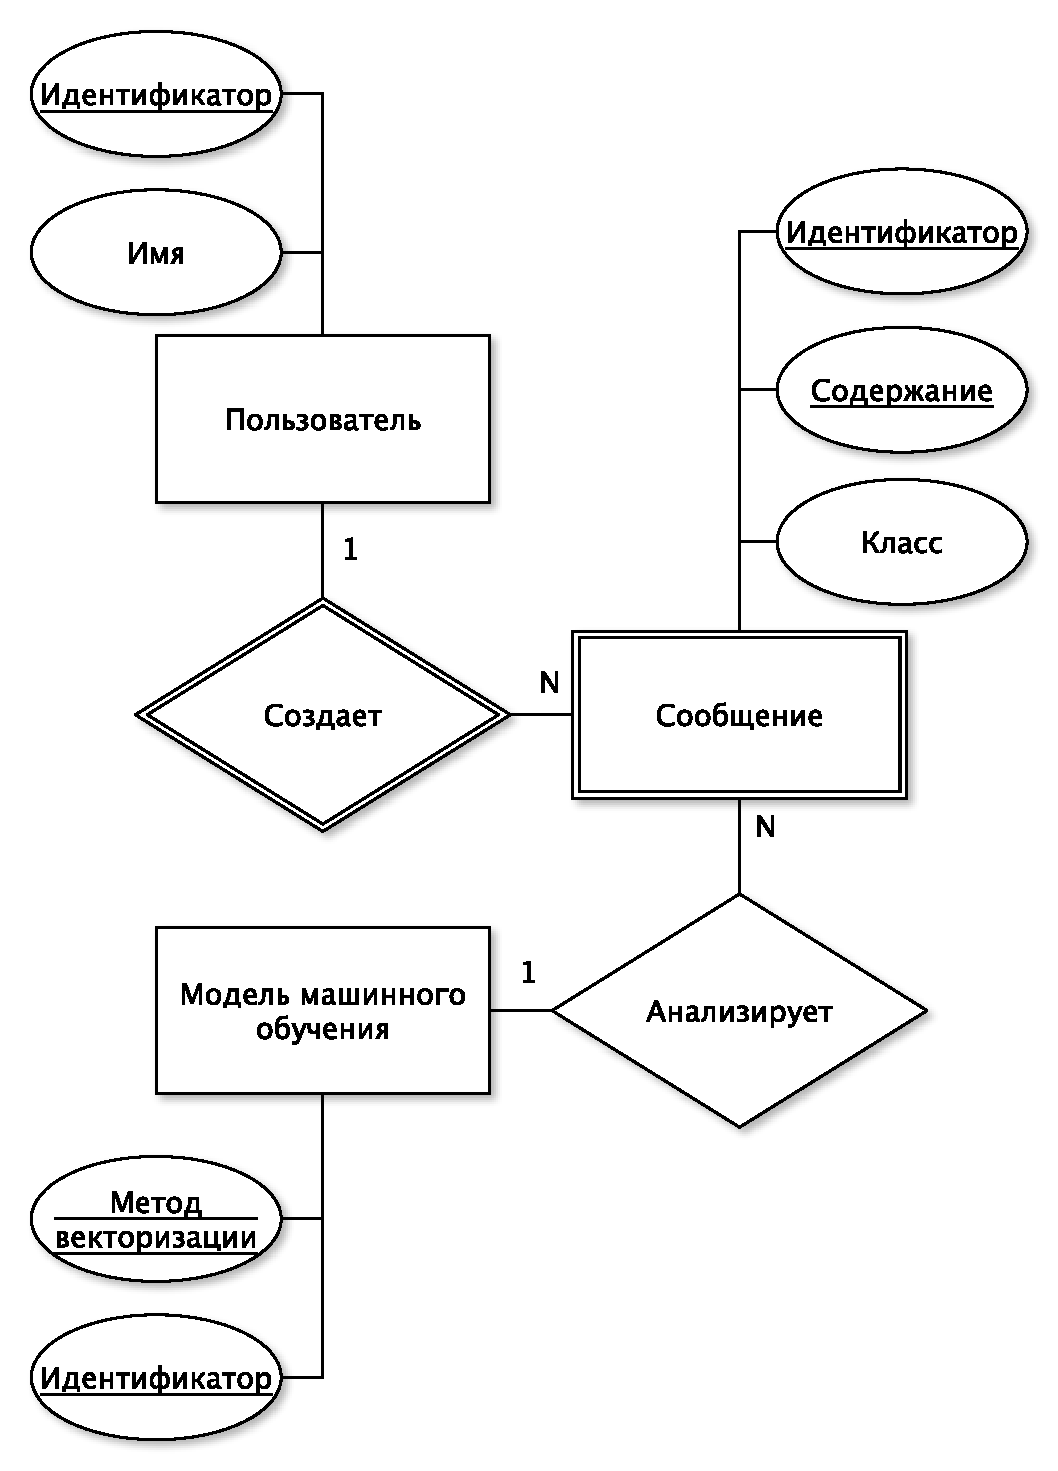
\includegraphics[width=\textwidth]{inc/er.pdf}
	\caption{ Диаграмма ``сущность-связь'' в нотации Чена. }
	\label{img:er}
\end{figure}



\subsection{Методы машинного обучения}

В качестве задействованных в методе алгоритмов рассматриваются: градиентный бустинг (схема алгоритма представлена на рисунке \ref{img:schemeGradient}), метод случайного леса (схема алгоритма представлена на рисунке \ref{img:schemeRandom}), метод опорных векторов (схема алгоритма представлена на рисунке \ref{img:schemeSvm}), метод К-ближайших соседей (схема алгоритма представлена на рисунке \ref{img:schemeKnn}), логистическая регрессия (схема алгоритма представлена на рисунке \ref{img:schemeLogistic}) и перцептрон (схема алгоритма представлена на рисунке \ref{img:schemePerceptrone}). Данный список обусловлен потребностью в целях исследования охватить широкий спектр методов машинного обучения для дальнейшего изучения возможности и потребности в создании ансамблевых моделей для решения поставленной задачи.

\begin{figure}[H]
	\centering
	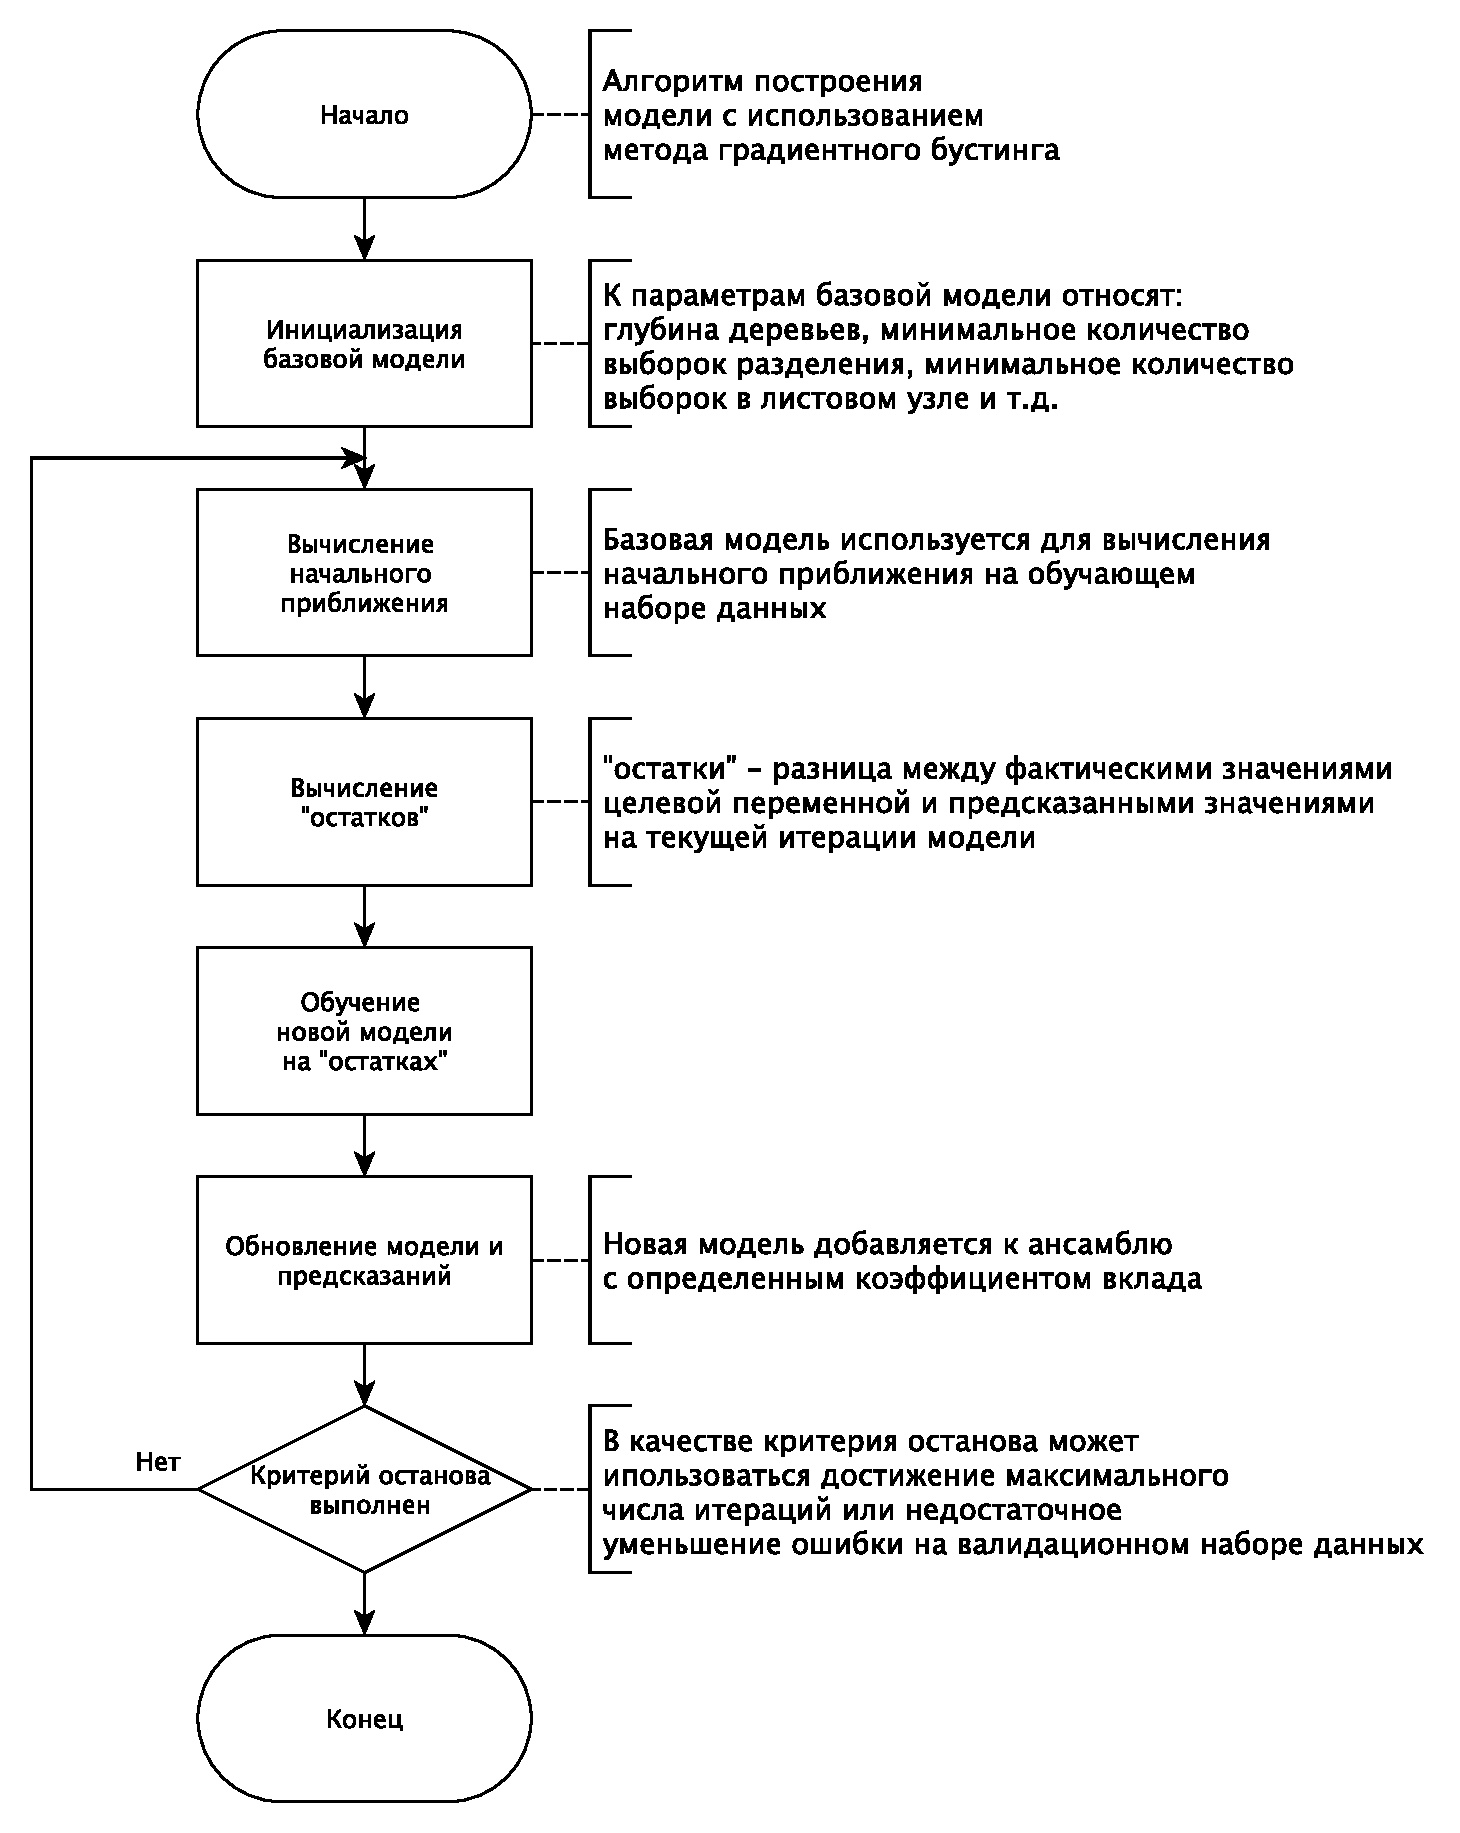
\includegraphics[width=\textwidth]{inc/schemeGradient.pdf}
	\caption{ Схема алгоритма работы градиентного бустинга. }
	\label{img:schemeGradient}
\end{figure}

\begin{figure}[H]
	\centering
	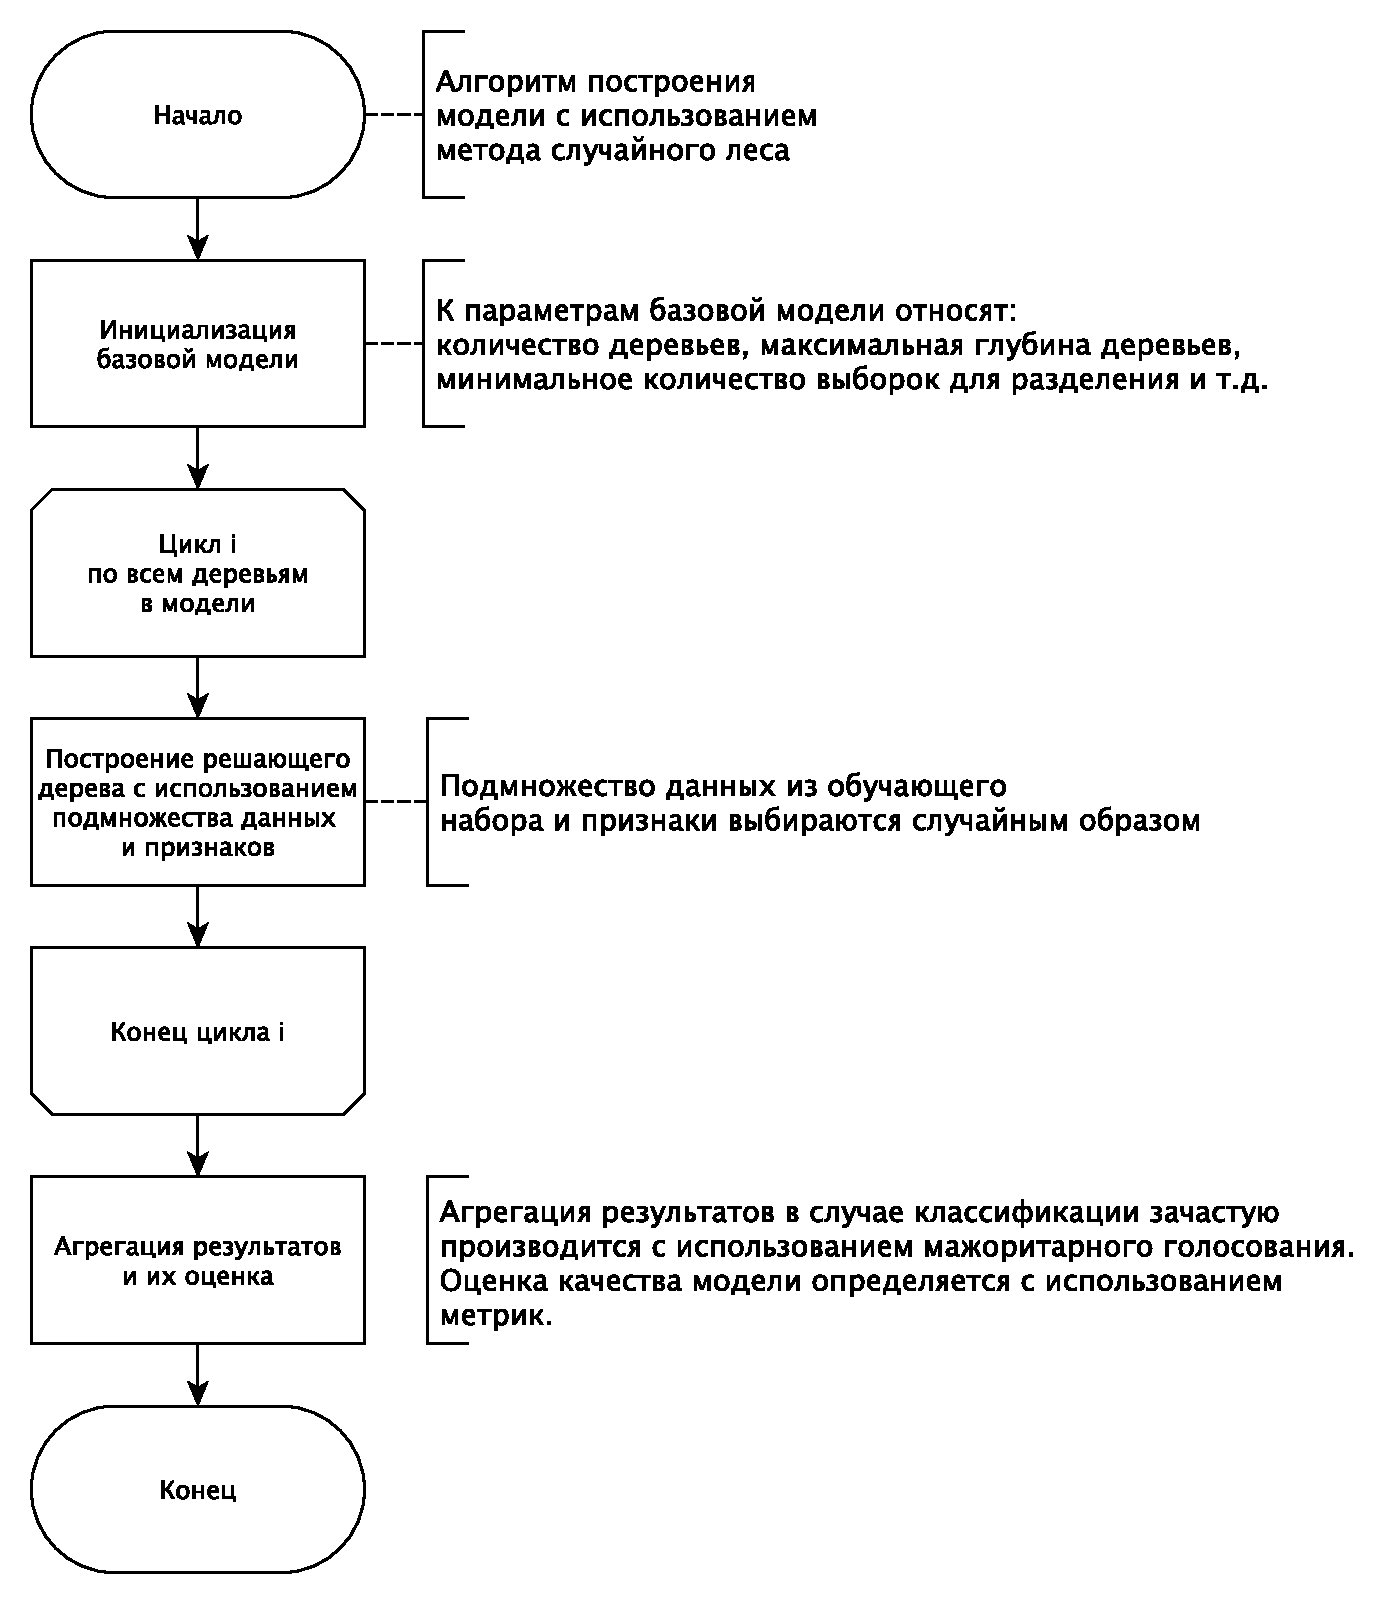
\includegraphics[width=\textwidth]{inc/schemeRandom.pdf}
	\caption{ Схема алгоритма работы метода случайного леса. }
	\label{img:schemeRandom}
\end{figure}

\begin{figure}[H]
	\centering
	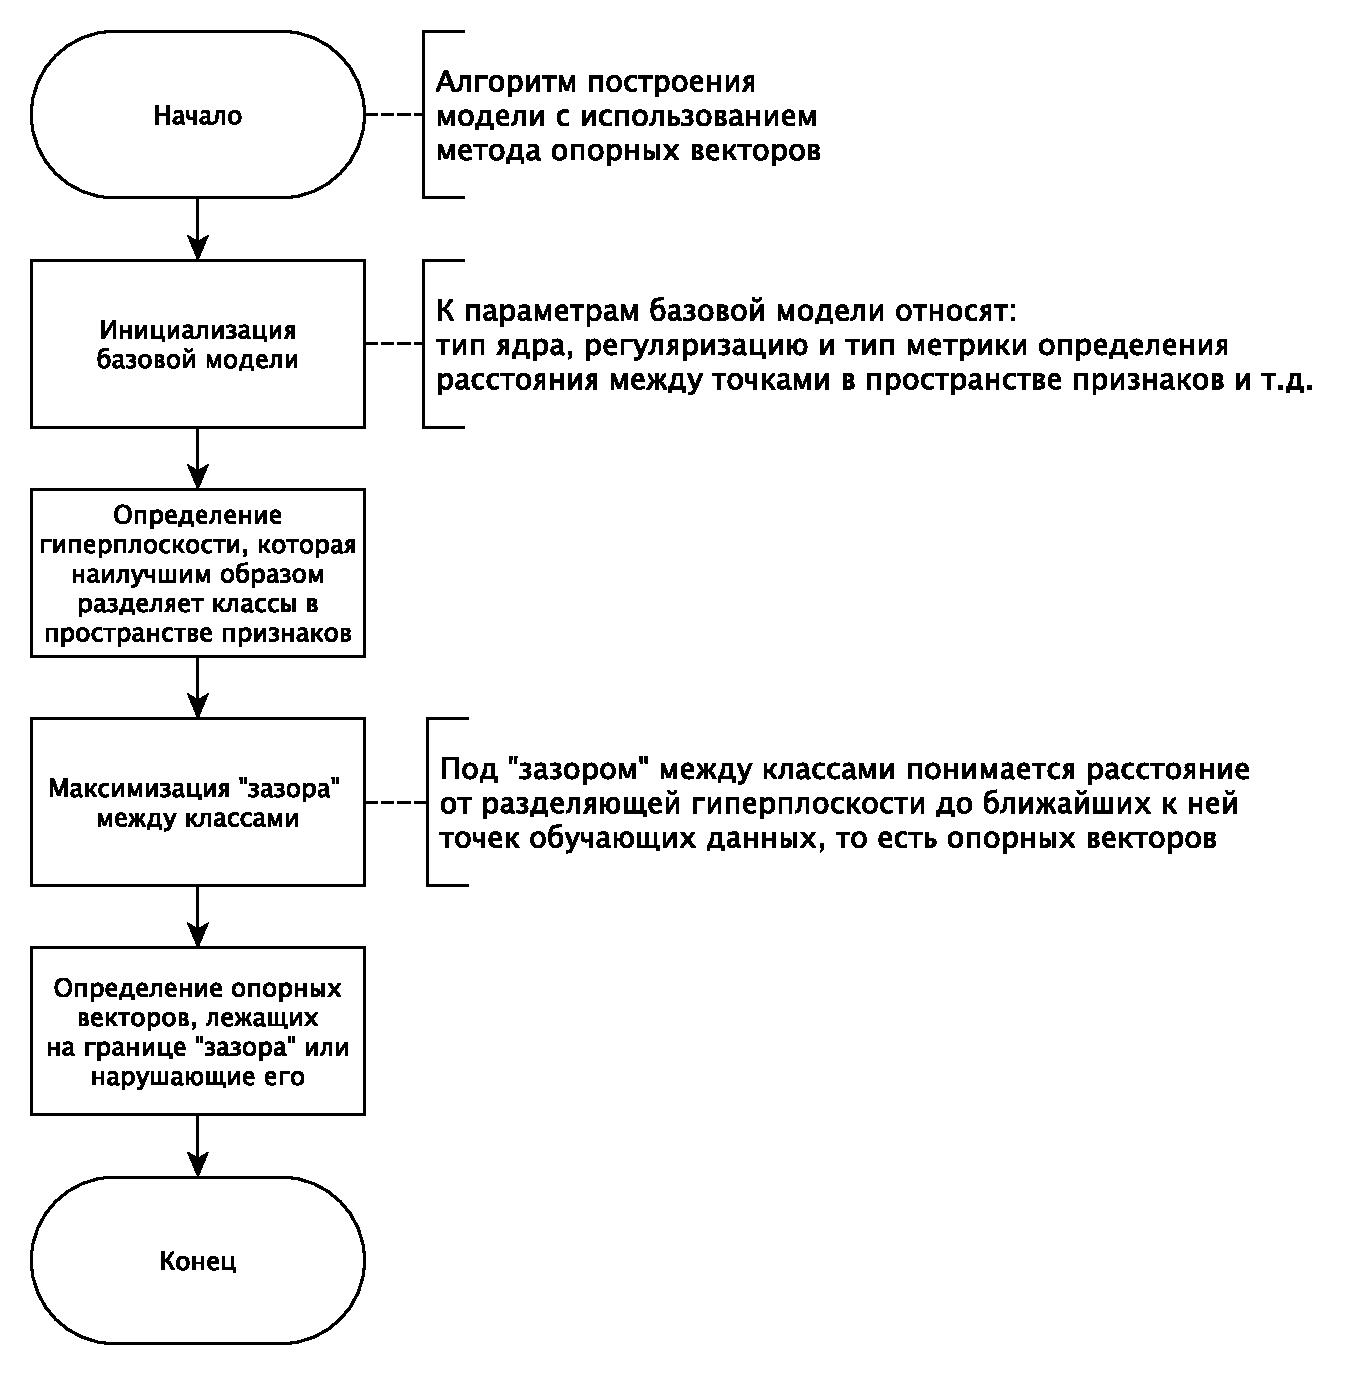
\includegraphics[width=0.7\textwidth]{inc/schemeSvm.pdf}
	\caption{ Схема алгоритма работы метода опорных векторов. }
	\label{img:schemeSvm}
\end{figure}

\begin{figure}[H]
	\centering
	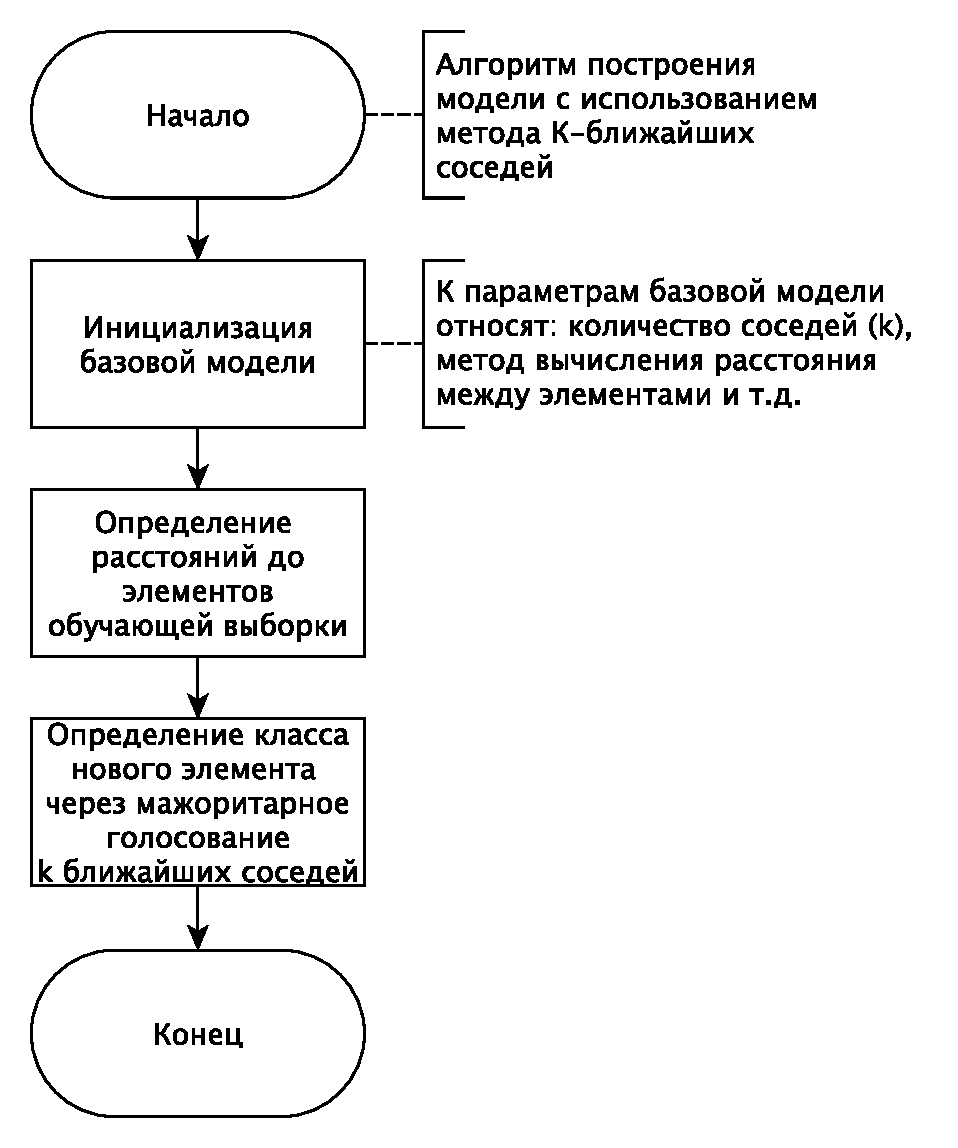
\includegraphics[width=0.7\textwidth]{inc/schemeKnn.pdf}
	\caption{ Схема алгоритма работы метода K-ближайших соседей. }
	\label{img:schemeKnn}
\end{figure}

\begin{figure}[H]
	\centering
	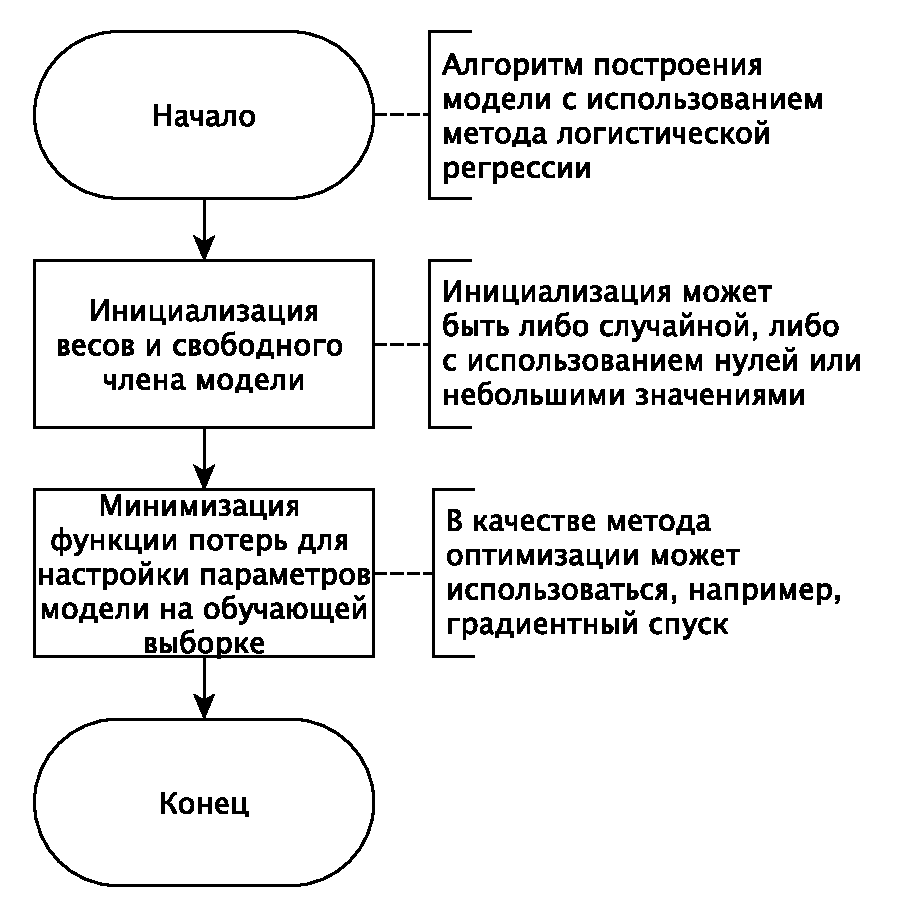
\includegraphics[width=0.7\textwidth]{inc/schemeLogistic.pdf}
	\caption{ Схема алгоритма логистической регрессии. }
	\label{img:schemeLogistic}
\end{figure}

\begin{figure}[H]
	\centering
	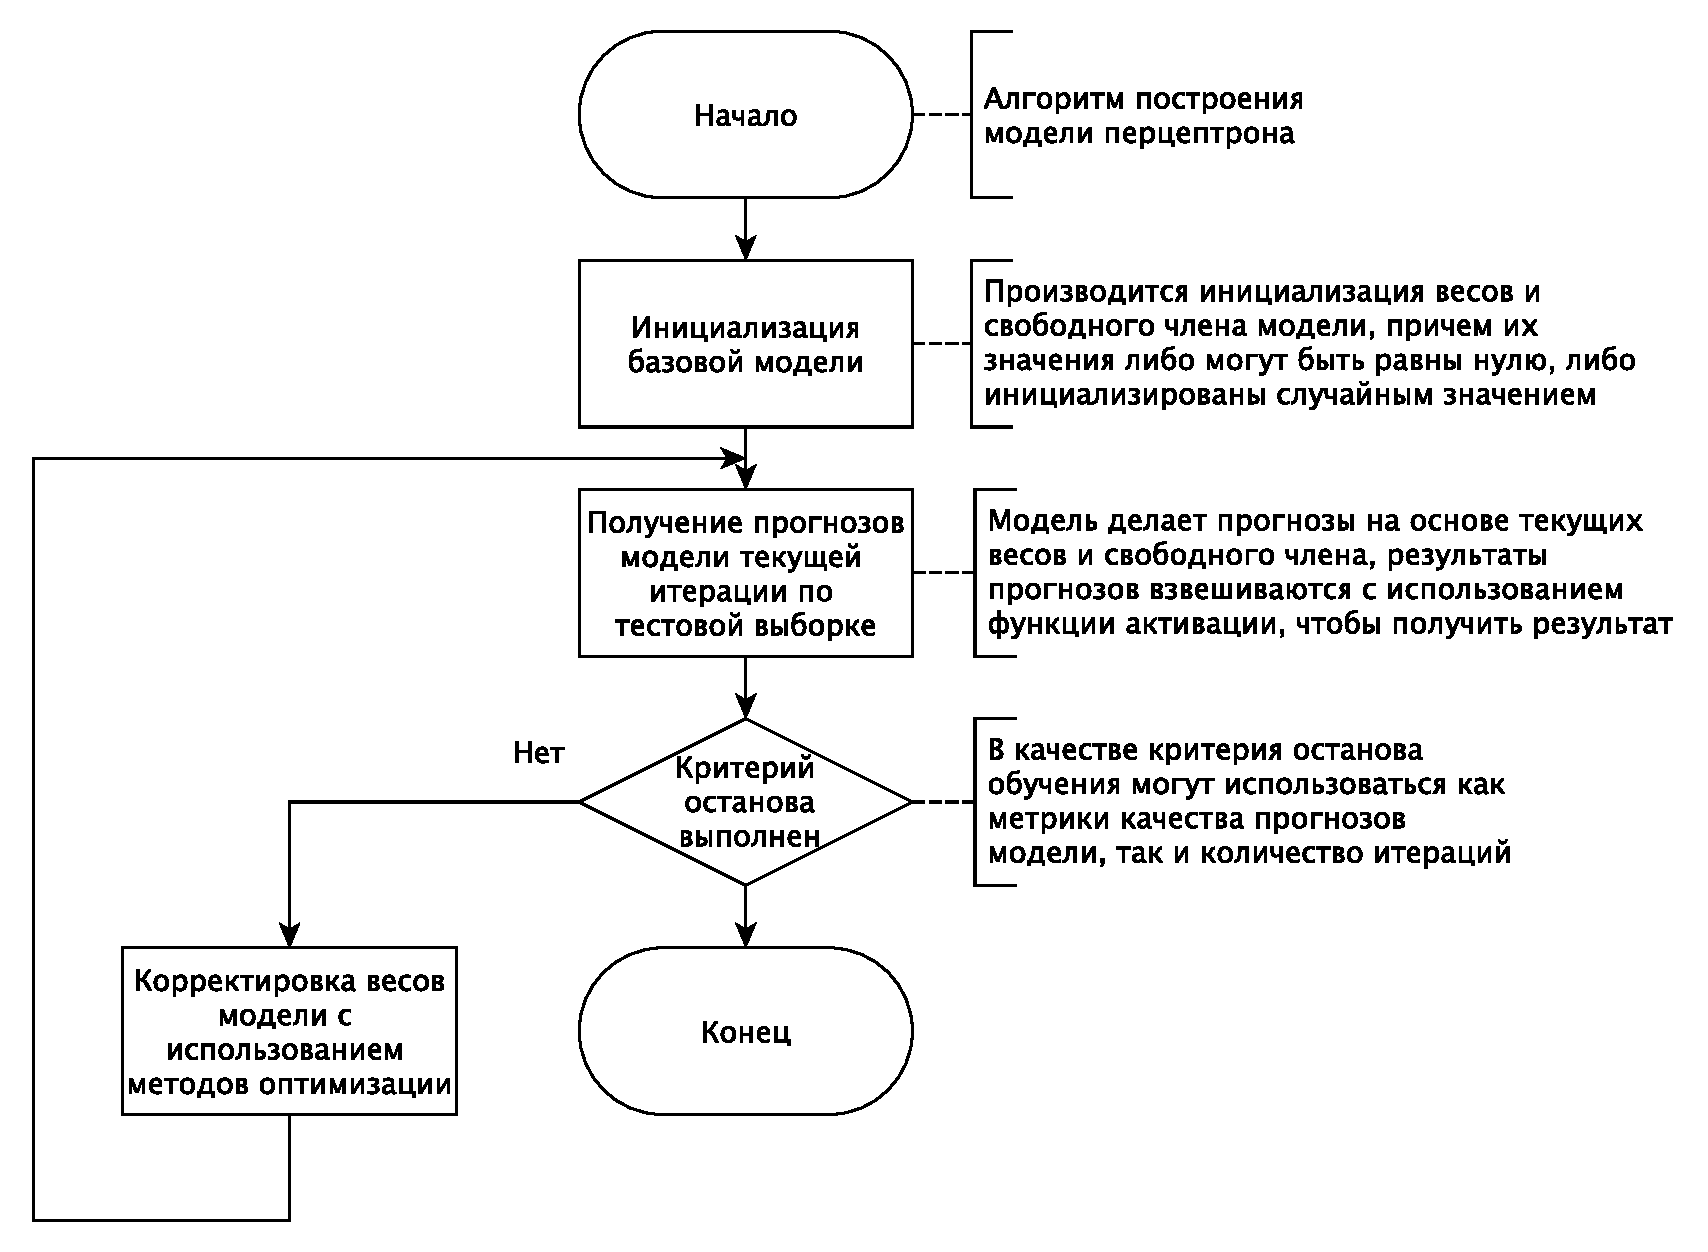
\includegraphics[width=\textwidth]{inc/schemePerceptrone.pdf}
	\caption{ Схема алгоритма работы метода с использованием перцептрона. }
	\label{img:schemePerceptrone}
\end{figure}

\subsection{Алгоритмы векторизации текстовых сообщений}

Для векторизации собранных текстовых сообщений будут задействованы алгоритм ``мешок слов'' и языковая модель BERT \cite{bert}.
Схемы работы выбранных алгоритмов представлены на рисунках \ref{img:schemeBagOfWords} и \ref{img:schemeBert} соответственно.
Алгоритм TF-IDF не входит в рассмотрение в силу того, что он является модернизацией алгоритма ``мешок слов''. 
Модели Word2Vec \cite{word2vec} и GloVe \cite{glove} также не попадают в рассмотрение в связи с тем, что данная работа первично имеет цель определить наиболее подходящий для решения задачи алгоритм машинного обучения.

\begin{figure}[H]
	\centering
	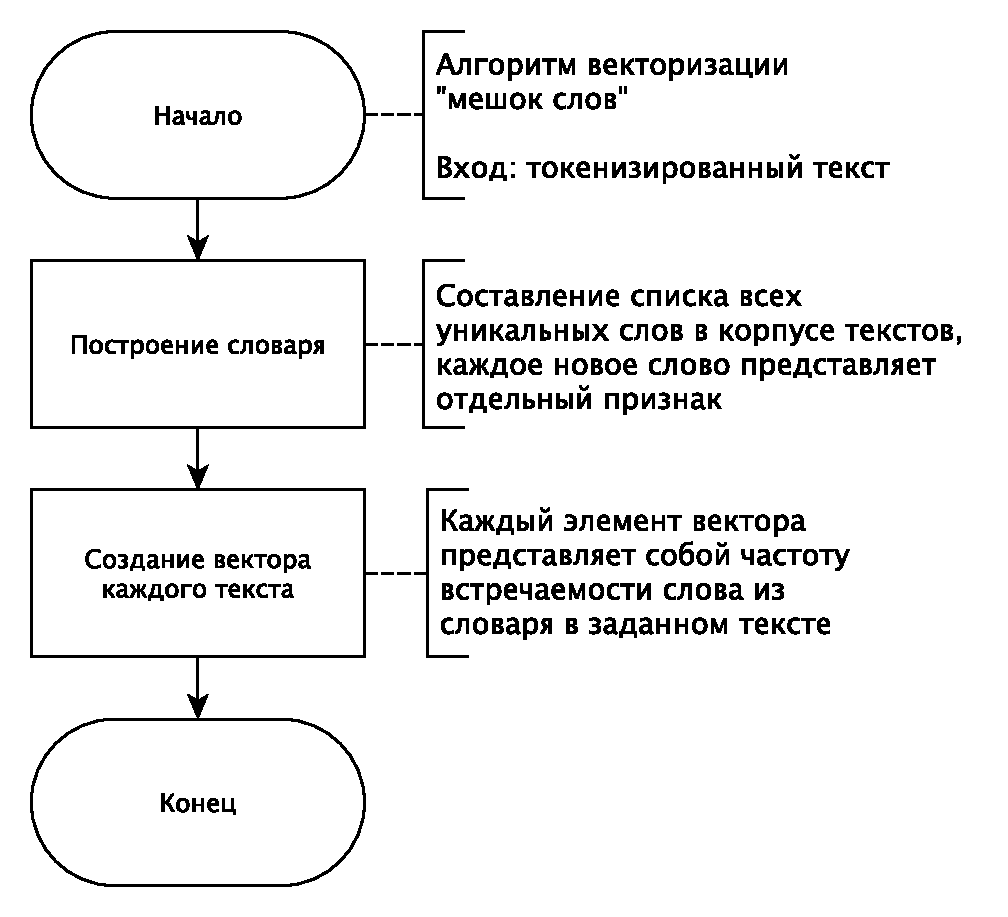
\includegraphics[width=0.5\textwidth]{inc/schemeBagOfWords.pdf}
	\caption{ Схема работы алгоритма ``мешок слов''. }
	\label{img:schemeBagOfWords}
\end{figure}

\begin{figure}[H]
	\centering
	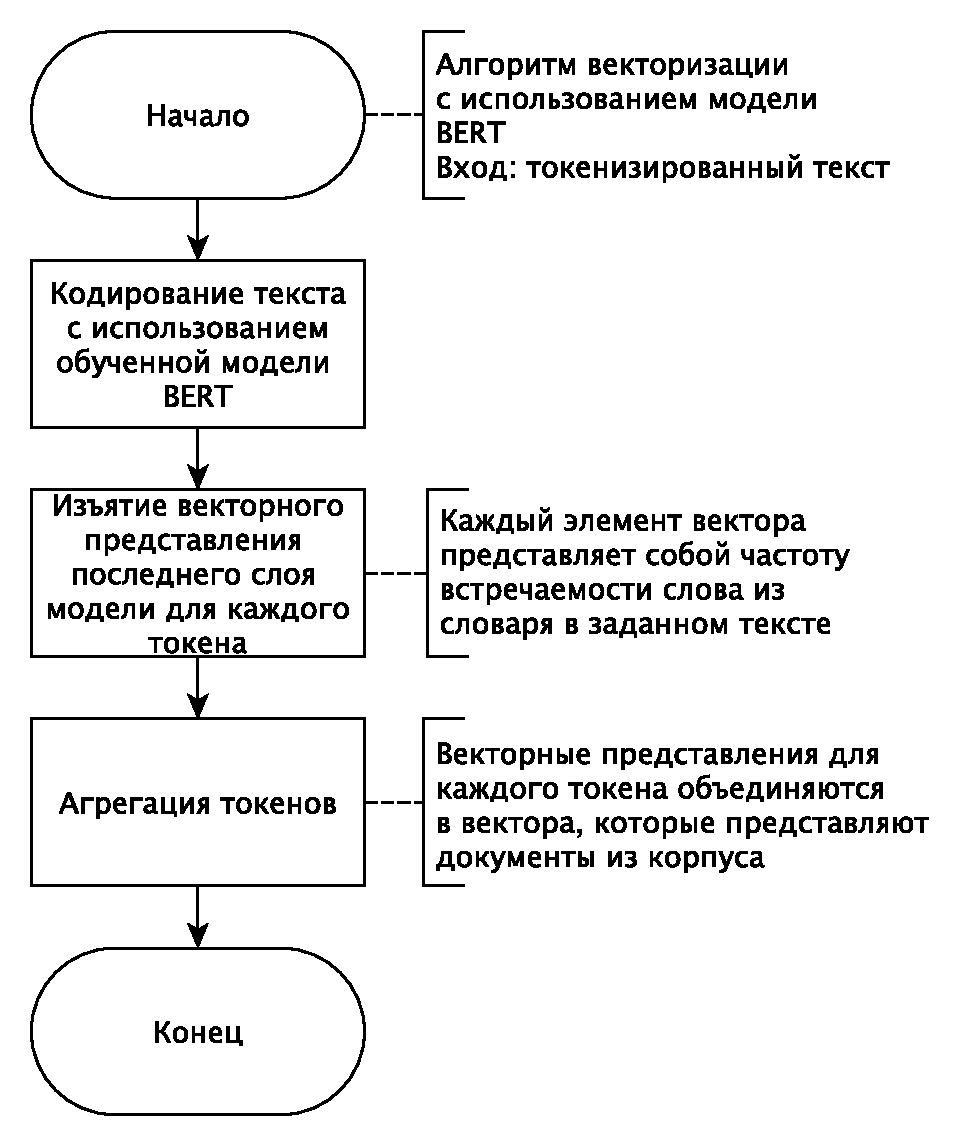
\includegraphics[width=0.4\textwidth]{inc/schemeBert.pdf}
	\caption{ Схема алгоритма векторизации с использованием модели BERT. }
	\label{img:schemeBert}
\end{figure}

\subsubsection*{Вывод}

Был описан метод распознавания суицидальных паттернов поведения человека по текстовым сообщениям, а также формат и метод сбора задействованных в нем данных. 
Определено, что в качестве средства сбора данных будет использоваться бот в мессенджере Telegram. Рассмотрены доступные средства реализации ботов в выбранном мессенджере.

Приведена диаграмма вариантов использования. Для системы было определено три действующих лица: пользователь, рекомендатор и анализатор. 
Приведена IDEF0 диаграмма, декомпозирована главная задача метода -- распознавание суицидального сообщения. 
Диаграмма ``сущность-связь'' в нотации Чена позволила на абстрактном уровне описать систему распознавания. 

Был определен перечень задействованных методов машинного обучения, который включил в себя: градиентный бустинг, метод случайного леса, метод опорных векторов, метод K-ближайших соседей, логистическая регрессия и перцептрон. В качестве методов векторизации выбраны: алгоритм ``мешок слов'' и языковая модель BERT.



\pagebreak